\documentclass[10pt]{article}
\usepackage{icmlko}

\icmlmeta{IP 파운데이션 월드모델}{273}{진짜로 돌려 봤다}{스무 노트를 손으로 짠 확인 스크립트로만 재고 실제 실행 경로를 안 돌렸다 --- 돌리니 셋이 나왔다}

\begin{document}

\twocolumn[
\icmlheader

\begin{abstract}
노트 253부터 272까지 스무 노트 동안 가드 · \texttt{rank} · \texttt{harness} ·
\texttt{provenance} · \texttt{fixaxes} 를 고쳤는데, 확인은 전부 \textbf{그때그때
손으로 짠 스크립트}로 했다. 실제 실행 경로(\texttt{python3 -m lab.loop})는
한 번도 안 돌렸다. 돌렸더니 셋이 나왔다. \textbf{첫째, 숨어 있던 경고.}
\texttt{tagaxes} 가 \texttt{matmul} 에서 divide-by-zero · overflow 를 띄우고
있었는데 내 확인 명령이 전부 \texttt{grep -v Warning} 으로 걸러내고 있었다.
파 보니 결과는 멀쩡하고(여섯 축 다 유한 100\%) 행렬곱에 나눗셈이 없으니
numpy SIMD 커널의 알려진 잡음이다 --- 그 한 줄에서 그 셋만 좁게 막았다.
\textbf{둘째, 죽어 있던 규약.} \texttt{evaluate} 의 \texttt{all} 갈래가
\texttt{Input y contains NaN} 으로 죽고 있었다. 노트 210이 게임 라벨을
30일 창으로 바꾸며 창이 안 찬 43건을 결측으로 뒀는데 그 갈래가 안 거른다.
\texttt{deploy} 갈래는 연도로 자르다 \emph{우연히} 같이 걸렀다 --- 그 43건이
전부 2025년 이후라서다. 승격은 안 막혔지만(가드 양규약이 ``전체 규약 없음''
으로 통과) 노트 112가 만든 \textbf{낙관 편의}를 그동안 못 재고 있었다.
\textbf{셋째, 그리고 이게 제일 크다.} \texttt{\_score\_one} 이 예측만 유한한지
보고 \emph{라벨은 안 본다}. 그래서 게임 점수가 \textbf{$+$0.19 로 저장되고
있었다 --- 옳은 값은 $+$0.62}다. 노트 271이 ``오래된 코드는 이 자리에서 안
틀린다''고 적었는데 \textbf{그게 반례다.} 다행히 순위 기준(\texttt{rank\_key}
$\to$ \texttt{guards.\_pooled} $\to$ \texttt{\_rho})은 둘 다 걸러서 챔피언
추적은 무사하다. 고친 김에 낙관 편의를 다시 쟀다 --- \textbf{F18 나무가
$+$0.18$\sim$0.20, F21 능형이 $+$0.03 으로 여섯 배 차이인데 축이 5 에서
23 으로 늘어도 안 커진다.} 축을 더한 것이 외우기를 사 온 게 아니다.
\end{abstract}
]

\section{스무 노트 만에}

노트 253--272 동안 고친 것을 세어 보면 가드 둘 추가(쌓임 · 겹말) · 가드 하나
수정 · \texttt{rank} 함수 둘 추가(\texttt{spread} · \texttt{clock}) ·
\texttt{harness} 에 \texttt{rows} 추가 · \texttt{provenance} 표 셋 ·
\texttt{fixaxes} 에 \texttt{BLOCK} · \texttt{tagaxes} 신규다.

\textbf{확인은 전부 손으로 짠 스크립트로 했다.} 축을 만들고 판을 재고 가드를
불러 보는 스무 줄짜리를 매번 새로 썼다. 그것이 통과하면 넘어갔다.
\texttt{lab.loop} 는 한 번도 안 돌렸다.

돌렸다.

\section{첫째 --- 내 명령이 경고를 지우고 있었다}

\begin{quote}\small
\texttt{tagaxes.py:193: RuntimeWarning: divide by zero encountered in matmul}
\end{quote}

내 확인 명령은 늘 \texttt{2>\&1 | grep -v Warning} 으로 끝났다. 한글 출력에서
numpy 경고를 걷어내려던 것인데, \textbf{그 필터가 ``RuntimeWarning'' 도 같이
지운다.}

파 봤다. \textbf{행렬곱에는 나눗셈이 없다.} 입력도 출력도 유한하고(여섯 축
전부 유한 100\% · 값 범위 $[0,1]$ · 서로 다른 값 140$\sim$2,012), numpy SIMD
커널이 안 쓰는 레인에서 부동소수 플래그를 세우는 알려진 잡음이다. 토큰
행렬이 순위 결손이라(원핫 열이 상수합) 특잇값에 $7{\times}10^{-14}$ 가 섞이는데
그것도 투영에는 해가 없다.

\texttt{np.errstate} 로 \textbf{그 한 줄에서 그 셋만} 막았다. 넓게 막으면
다음 진짜 경고를 또 못 본다.

\section{둘째 --- 규약 하나가 죽어 있었다}

\begin{quote}\small
\texttt{error: all 실패: ValueError Input y contains NaN.}
\end{quote}

\texttt{harness.evaluate} 의 \texttt{all} 갈래는 이랬다.

\begin{center}\small
\begin{verbatim}
f = make(); f.fit(data)   # 라벨 NaN 포함 전부
\end{verbatim}
\end{center}

노트 210이 게임 라벨을 누적 리뷰에서 \textbf{30일 창}으로 바꾸면서 창이 안 찬
43건을 결측으로 뒀다. 그 43건이 그대로 들어간다.

\texttt{deploy} 갈래는 왜 멀쩡했나. 연도로 자르는데 \textbf{그 43건이 전부
2025년 이후}라 우연히 같이 걸렸다. \emph{우연히 안 죽은 것이지 옳았던 게
아니다.}

승격은 안 막혔다 --- 가드 \textbf{양규약}이 전체 규약 점수가 없으면
``전체 규약 없음''으로 통과한다. 대신 노트 112가 보라고 만든 \textbf{낙관
편의}(전체 $-$ 배포)를 노트 210 이후로 못 재고 있었다.

\section{셋째 --- 게임 점수가 $+$0.19 였다}

\begin{figure}[t]
\centering
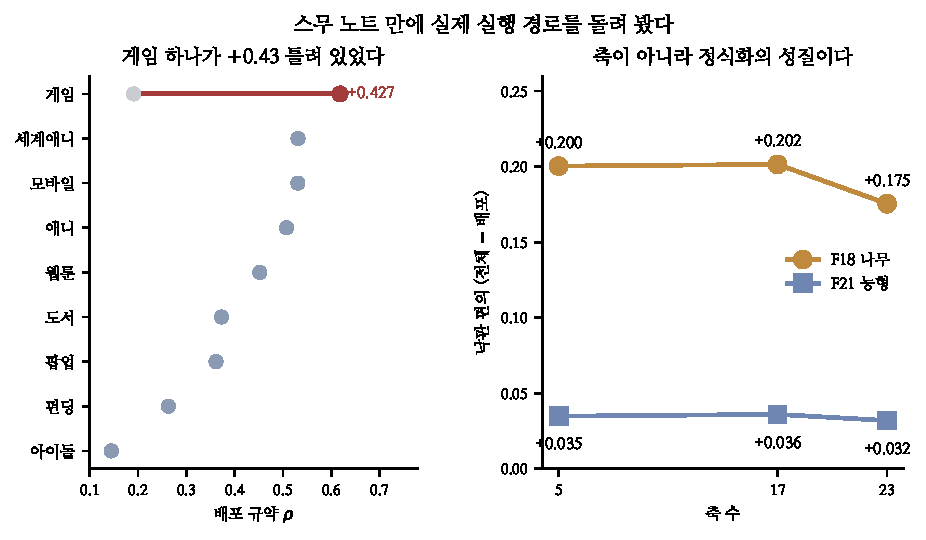
\includegraphics[width=\columnwidth]{figs/run.pdf}
\caption{왼쪽 --- 고치기 전후의 배포 점수. 오른쪽 --- 낙관 편의.}
\end{figure}

루프가 저장한 배포 점수를 보다가 게임이 \textbf{$+$0.1911} 인 것을 봤다.
같은 판에서 내 \texttt{rank.pooled} 은 게임을 $+$0.62 로 잰다. 씨앗 차이로는
설명이 안 되는 폭이다.

\begin{center}\small
\begin{verbatim}
ok = np.isfinite(p)             # 예측만 본다
return float(spearman(p[ok], y[ok]))
\end{verbatim}
\end{center}

\textbf{라벨을 안 본다.} 게임의 결측 라벨 43건이 순위에 들어가 상관을
망가뜨린다. 고치니 \textbf{$+$0.1911 $\to$ $+$0.6184}, 배포 평균이 0.3727에서
0.4202 가 된다.

\paragraph{노트 271이 틀렸다} 나흘 전 노트 271에 이렇게 적었다 --- ``셋 다
새로 쓴 재는 코드에서 났다. 오래된 코드는 안 틀린다.''
\texttt{harness.\_score\_one} 은 이 판에서 제일 오래된 코드에 속하고
\textbf{같은 병에 걸려 있었다.} 네 번째다.

\paragraph{다행인 것} 순위 기준은 무사하다. \texttt{rank\_key} 는
\texttt{guards.\_pooled} 의 값을 쓰고 그것은 \texttt{\_rho} 를 부르는데,
\texttt{\_rho} 는 \texttt{np.isfinite(p) \& np.isfinite(y)} 로 \textbf{둘 다}
거른다. 그래서 챔피언 추적과 판 수는 영향이 없다. 망가진 것은
\texttt{scores} 표에 저장된 도메인 점수와, 승격의 동점 깨기가 읽는
\texttt{\_per\_target} 의 게임 열이다.

\section{고친 김에 --- 낙관은 축이 아니라 형식이다}

\begin{center}\small
\begin{tabular}{lrrrr}
\hline
축 & F18 배포 & F18 낙관 & F21 낙관 & 비 \\
\hline
5 (base) & 0.3245 & $+$0.2004 & $+$0.0348 & 5.8 \\
17 (trendcalwiki) & 0.4097 & $+$0.2015 & $+$0.0360 & 5.6 \\
23 (지금) & 0.4202 & $+$0.1755 & $+$0.0319 & 5.5 \\
\hline
\end{tabular}
\end{center}

\textbf{나무가 능형의 여섯 배쯤 낙관적이고, 축을 5 에서 23 으로 늘려도 안
커진다} --- 오히려 23축에서 조금 내린다($+$0.2015 $\to$ $+$0.1755). 시간을
안 가르면 나무는 0.18$\sim$0.20 을 더 받고 능형은 0.03 을 더 받는다 ---
외우는 능력의 차이다.

여기서 읽을 것은 \textbf{축 추가가 외우기를 사 오지 않았다}는 것이다. 노트
255 · 257 · 260이 넣은 축 여섯이 낙관을 한 자리도 안 올렸다. 판이 오른
$+$0.0276 은 시간을 갈라서 잰 값이고 그 값은 그대로다.

\paragraph{남은 것}
\begin{center}\small
\begin{tabular}{ll}
\hline
갈래 & 왜 \\
\hline
저장된 점수 & 노트 210 이후 게임 열이 다 틀렸다. 다시 돌릴까 \\
동점 깨기 & \texttt{\_per\_target} 이 그 열을 읽는다 \\
루프를 자주 & 스무 노트에 한 번은 너무 드물다 \\
낙관 0.18 & 나무가 그만큼 외운다. 줄일 길이 있나 \\
\hline
\end{tabular}
\end{center}

\paragraph{규약} \textbf{손으로 짠 확인은 실제 실행 경로를 대신하지 못한다.}
그리고 확인 명령에서 \textbf{경고를 지우지 않는다} --- 이번에 셋 중 하나를
그것 때문에 놓칠 뻔했다. 노트 253 · 259 · 261 · 267 · 270의 한 줄짜리
검정들에 여섯 번째를 붙인다: \textbf{가끔은 그냥 진짜로 돌려 본다.}

\end{document}
